Pour donner un exemple d'œuvre contemporaine, le schéma d'installation de la pièce \textit{Fluoresce} (R. Gottfried, 2012) est présentée en figure \ref{fig:schemaInstallationFluoresce}.

\begin{figure}[H]
	\centering
	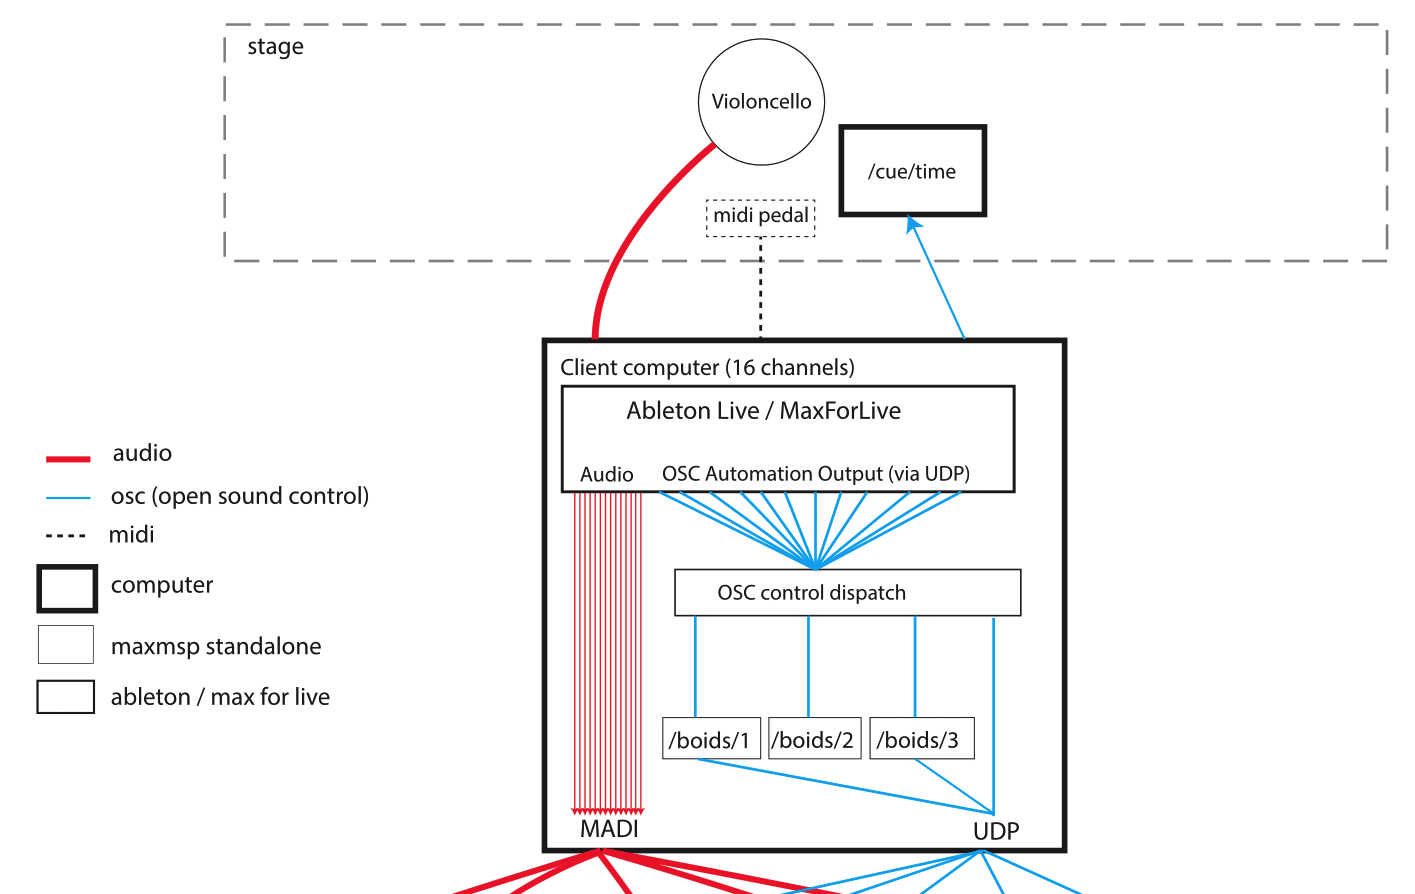
\includegraphics[keepaspectratio=true, width=\textwidth]{Notation/i/schemaInstallationFluoresce.png}
	\caption[Schéma de branchement pour la pièce \textit{Fluoresce} par Rama Gottfried]{Schéma de branchement pour la pièce \textit{Fluoresce} par Rama Gottfried}
	\label{fig:schemaInstallationFluoresce}			
\end{figure}
\begin{center}
\small \it La figure \ref{fig:schemaInstallationFluoresce} présente le schéma de câblage des différents éléments qui vont servir à l'exécution de la pièce. La performance fait intervenir un joueur de violoncelle (\textit{Violoncello}); le son produit par le violoncelle est capté et envoyé à un ordinateur (\textit{Client computer}) sur lequel est lancé la station audionumérique\footnote{\og Une station audionumérique (acronyme DAW, de l'anglais digital audio workstation) désigne […] un ensemble d'outils électroniques, conçu pour enregistrer, éditer, manipuler, créer et lire des contenus audionumériques.\fg -- Wikipédia} \textit{Ableton Live} associé au plugin \textit{MaxForLive}\footnote{MaxForLive est un plugin permettant l'intégration du logiciel Max/MSP à la station audionumérique Ableton Live. Voir plus loin pour plus de détails sur Max/MSP.}. Ableton Live répartit le signal audio sur les systèmes WFS et HOA (\textit{Wave Field Synthesis} et \textit{High Order Ambisonics}\footnote{\textit{Wave Field Synthesis} et \textit{High Order Ambisonics} sont deux systèmes de diffusion de sons spatialisés basés sur l'utilisation d'un grand nombre d'enceintes.}) via la liaison MADI\footnote{MADI (Multichannel Audio Digital Interface) est une liaison audionumérique définissant un protocole capable d'embarquer 64 canaux audio simultanément}. Le plugin MaxForLive envoie des messages OSC\footnote{Open Sound Control. Protocole de communiaction entre ordinateurs, synthéthiseurs et autres appareils. \textbf{Voir le chapitre} pour plus de détails.} \texttt{/boids/1}, \texttt{/boids/2} et \texttt{/boids/3} (directives de déclenchement d'effets sonores), via UDP, aux systèmes WFS et HOA. Le schéma de branchement complet est consultable en annexe \ref{sec:schemaInstallationFluoresceComplet} page~\pageref{sec:schemaInstallationFluoresceComplet}. L'écoute et la description de la pièce \textit{Fluoresce} sont accessibles à l'url \url{http://www.ramagottfried.com/fluoresce.html}.
\end{center}

La pièce \textit{Fluoresce} est un type de musique appelée "musique mixte", c'est à dire qui mélange instruments traditionnels et Informatique temps-réel.
Sur le schéma, l'ordinateur sur scène envoie le message OSC \texttt{/cue/time} au \textit{Client computer}. Le message \texttt{/cue/time} transmet un référentiel temporel permettant la synchronisation entre le jeu du violoncelliste et le \textit{Client computer}. 
Dans le cas de musique mixte, la question de la synchronisation humain/machine et du suivi de partition est centrale. 
En effet, même si une pièce de musique contemporaine peut se détacher de toutes notions de métrique, de mélodie et d'harmonie, elle admet tout de même un ordonnancement temporel des éléments la composant.
D'ailleurs, sur les partitions du XXème siècle, Jean-Yves Bosseur indique que la notation agit comme le \og déclencheur d'une chaîne d'actions et de réactions sonores \fg (\cite[121]{bosseur2005}), illustrant bien l'impératif de temporisation et de synchronisation inhérent à la musique contemporaine.
